\begin{figure}
  \centering
  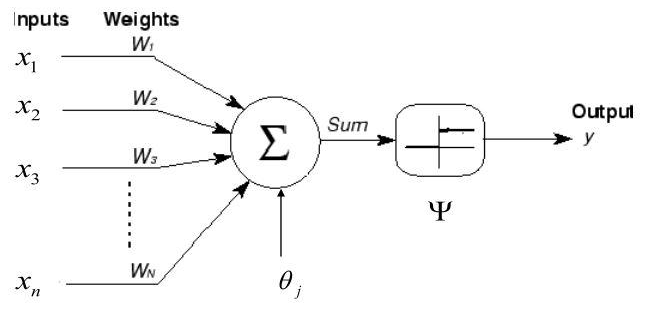
\includegraphics[width=8cm]{./Chapitre2/figures/perceptron.png}
  \caption{Représentation schématique d'un perceptron. $X_i$ correspond aux entrées, $W_i$ correspond aux poids associés à chacune des entrées $X_i$, \theta formalise le biais. Une fois sommée, la valeur est passée dans une fonction d'activation pour déterminer la valeur de sortie.}
  \label{fig:perceptron}
\end{figure}
